%%%%%%
%
% $Autor: Wings $
% $Datum: 2020-01-18 11:15:45Z $
% $Pfad: WuSt/Skript/Produktspezifikation/powerpoint/ImageProcessing.tex $
% $Version: 4620 $
%
%%%%%%

%todo WS: CNN heraus

\chapter{Prozesse zur Wissensgewinnung in Datenbanken}

\section{Knowledge Discovery in Databases (KDD-Prozess)}

Die Wissensfindung in Datenbank, englisch Knowledge Discovery in Databases, kurz KDD, ist der entscheidende Schritt bei der Betrachtung von Daten. Es existieren verschiedene Möglichkeiten der Wissensfindung. Um jedoch effizient und systematisch das Ziel zu erreichen, ist ein geeigneter Prozess in immanenter Wichtigkeit. In diesem Abschnitt wird der KDD-Prozess detailliert betrachtet. In diesem Prozess wird die Wissensfindung in mehrere Schritte unterteilt.  \cite{Dusing.2000}

\subsection{Anwendungsgebiete}
Der KDD-Prozess kann grundsätzlich immer dann angewendet werden, wenn große Datenmengen zur Verfügung stehen, aus denen Wissen extrahiert werden kann. Der KDD-Prozess wurde in dem Artikel von Fayyad dargestellt. \cite{Fayyad:1996}  Dort werden als Beispiele zu Anwendungsgebieten die Bereiche Astronomie, Investment, Marketing, Betrugserkennung, Herstellungsprozesse und Telekommunikation genannt. Doch auf diese Gebiete ist der KDD-Prozess nicht beschränkt. So präsentiert \cite{Maimon:2010} verschiedene Anwendungen in den Bereichen Finanzen, Medizin, Erkennung von Angriffen auf Computersysteme oder Customer-Relationship-Management. Wenngleich bei diesen Beispielen alle Elemente des des KDD-Prozesses detailliert ausgeschöpft werden, zeigt Anwendung auf diesen Gebieten den möglichen Einsatz des gesamten KDD-Prozesses mit Data Mining als Kernelement auf. \cite{Pyo:2002} beschreibt die Anwendung des KDD-Prozesses auf Datensätze zu touristischen Reisezielen, die etwa zu Erkenntnissen zu Möglichkeiten der Attraktivitätssteigerung einzelner Reiseziele führen kann.

Die genannte Literatur zeigt die vielseitige Einsetzbarkeit des KDD-Prozesses auf. Grundsätzlich kann er überall eingesetzt werden, wo genügend Daten zur Verfügung stehen und einer Generalisierung gewisser Strukturen zulässig ist. 


\subsection{Prozessmodell}

Eine Schwierigkeit bezüglich des KDD-Prozesses ist, dass \glqq derzeit kein generelles Vorgehensmodell des Knowledge Discovery in Databases verfügbar ist \grqq \cite{Dusing.2000}. Es gibt verschiedene Modelle, die den Prozessschritte ausgehend von den Daten hin zum extrahierten Wissen darstellen.  Eines der ersten und laut \cite{Kurgan:2006} das meistzitierte Model ist das nach  Fayyad \cite{Fayyad:1996}. Daher soll dieses im Folgenden dargestellt werden. Laut \cite{Kurgan:2006} sind es vor allem der KDD-Prozess nach Fayyad und CRISP-DM, die auch im  technischen/ingenieurwissenschaftlichen Bereich Anwendung finden, während viele der anderen Modelle eher auf Bereiche im und um das Marketing abzielen. Deshalb sollen beide (Fayyad und CRISP-DM) beschrieben werden.  Dazu wird ein generisches Modell und ein solches auf die Anwendung mit Edge Computern ausgelegtes Modell vorgestellt.

\subsection{KDD-Prozess nach Fayyad}
Auf abstrakter Ebene beschäftigt sich das Feld des KDD mit der Entwicklung von Methoden und Techniken um \glqq aus Daten Sinn zu machen\grqq \cite{Fayyad:1996}. Dafür müssen mehrere Schritte durchlaufen werden. Zu beachten ist hierbei der iterative Charakter des Prozesses: Immer wieder kann und muss auf Grund der zugewonnenen Erkenntnisse zu den vorherigen Schritten zurückgekehrt und Korrekturen vorgenommen werden. Unter Umständen müssen weitere Daten beschafft oder andere Vorverarbeitungsschritte eingeführt werden. \cite{Wrobel:1998}

Der grundlegende Ablauf des KDD-Prozesses sowie die enthaltenen Iterationsschleifen sind in Abbildung~\ref{KDDFayyad} zu erkennen.

\begin{figure}[H]
	\begin{center}
        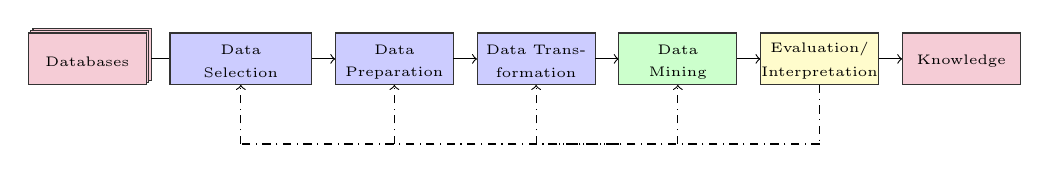
\begin{tikzpicture}[scale=0.6]
            \draw[draw, black!80, fill=blue!20!red!20]  (-2.90,0.10) rectangle (-0.40,1.20);
            \draw[draw, black!80, fill=blue!20!red!20]  (-2.95,0.05) rectangle (-.45,1.15);
            \draw[draw, black!80, fill=blue!20!red!20]  (-3,0) rectangle (-0.5,1.1);
            \node (AMP) at (-1.75,0.5) {\tiny Databases};
            
            %\visible<2->
            {
                \draw[->] (-0.4,0.55)--(1.5,0.55);
                \draw[draw, black!80, fill=blue!20]  (0,0) rectangle (3,1.1);
                \node (AMP) at (1.5,0.75) {\tiny Data};
                \node (AMP) at (1.5,0.25) {\tiny Selection};
            }
            
            %\visible<3->
            {
                \draw[->] (3,0.55)--(3.5,0.55);
                \draw[draw, black!80, fill=blue!20]  (3.5,0) rectangle (6,1.1);
                \node (AMP) at (4.75,0.75) {\tiny Data};
                \node (AMP) at (4.75,0.25) {\tiny Preparation};
            }
            
            
            %\visible<4->
            {
                \draw[->] (6,0.55)--(6.5,0.55);
                \draw[draw, black!80, fill=blue!20]  (6.5,0) rectangle (9,1.1);
                \node (AMP) at (7.75,0.75) {\tiny Data Trans-};
                \node (AMP) at (7.75,0.25) {\tiny formation};
            }
            
            %\visible<5->
            {
                \draw[dash dot,->] (10.75,-1.25)--(10.75,0);
                \draw[->] (9.0,0.55)--(9.5,0.55);
                \draw[draw, black!80, fill=green!20]  (9.5,0) rectangle (12,1.1);
                \node (AMP) at (10.75,0.75) {\tiny Data};
                \node (AMP) at (10.75,0.25) {\tiny Mining};
            }
           
            {
                \draw[->] (12,0.55)--(12.5,0.55);
                \draw[draw, black!80, fill=yellow!20]  (12.5,0) rectangle (15,1.1);
                \node (AMP) at (13.75,0.25) {\tiny Interpretation};
                \node (AMP) at (13.75,0.75) {\tiny Evaluation/};
            }
            
            \draw[->] (15,0.55)--(15.5,0.55);
            \draw[draw, black!80, fill=blue!20!red!20]  (15.5,0) rectangle (18,1.1);
            \node (AMP) at (16.75,0.5) {\tiny Knowledge};
            
            
            %\visible<8->
            {
                \draw[dash dot,-] (9.5,-1.25) -- (1.5,-1.25);
                \draw[dash dot,->] (1.5,-1.25)--(1.5,0);
            }
            
            %\visible<9->
            {
                \draw[dash dot,->] (4.75,-1.25)--(4.75,0);
                \draw[dash dot,->] (7.75,-1.25)--(7.75,0);
            }
            
            %\visible<2->
            {
                \draw[dash dot,-] (13.75,0)--(13.75,-1.25);
                \draw[dash dot,-] (13.75,-1.25) -- (8,-1.25);
                
            }
        \end{tikzpicture}
		\caption{KDD-Prozess nach \cite{Fayyad:1996} (eigene reduzierte Darstellung auf Grundlage von \cite{Fayyad:1996})} 
\label{KDDFayyad}
\end{center}
\end{figure}


    %  \GRAPHICSC{1.0}{1.0}{BigData/KDD}
    


Zu Beginn des KDD-Prozesses steht immer die verfügbare Datenbasis, aus der das Wissen gewonnen werden soll. Daraus müssen die zu verwendenden Daten aus einer oder mehreren Datenbanken ausgewählt und die Daten anschließend aufbereitet und vorbereitet werden. Erst dann können die Daten mit Hilfe von Data-Mining-Methoden zur Wissensextraktion verwendet werden. Nach der Auswertung und eventuell mehreren Durchläufen der verschiedenen Schritte kann das gewonnene Wissen schlussendlich extrahiert und in der Anwendung verwendet werden.

Fayyad unterteilt diesen Prozess weiter in neun Teilschritte, die zum Teil nicht direkt in Abbildung \ref{KDDFayyad} repräsentiert sind. Diese neun Schritte werden nachfolgend beschrieben.

\subsubsection{1. Domänenwissen} % (Developing an Understanding of the Application Domain)}

Zuerst muss die Domäne der Anwendung definiert und verstanden werden. Dazu gehört auch das für die Anwendung benötigte Domänenwissen, um die Analyse auf eine zu echtem Mehrwert führende Art durchführen zu können. Zudem müssen die genauen Ziele des KDD-Prozesses für den Anwendungsfall und den spezifischen Endnutzer des Wissens definiert werden \cite{Fayyad:1996,Kurgan:2006}. Dieser Schritt bildet die Grundlage, um die in den nächsten 
Schritten notwendigen Entscheidungen treffen zu können \cite{Maimon:2010}.

\subsubsection{2. Datensatz erstellen} % (Creating a Target Data Set)}

Als nächstes wird ein Datensatz oder eine Teilmenge eines Datensatzes ausgewählt. Dabei können einzelne oder mehrere Variablen ausgewählt werden, um die Daten, aus denen das Wissen entnommen werden soll, einzugrenzen. \cite{Fayyad:1996} Das beinhaltet die Feststellung, welche Daten verfügbar sind und eventuell die Beschaffung noch fehlender Daten. Dabei ist es wichtig, dass alle notwendigen Informationen enthalten sind. Die Entscheidung, welche Variablen notwendig sind, muss auf der Grundlage des Domainwissens erfolgen. Nach der Auswahl der Variablen sollten für ein gutes Modell möglichst viele Repräsentanten der Variablen dem Algorithmus zur Verfügung werden. Andererseits ist die Sammlung, Speicherung und Verarbeitung von größeren Datensätzen aufwendiger und viele Variablen können zudem zu schwer interpretierbaren Ergebnissen führen. Daher ist schon bei diesem Schritt die Relevanz der Rückkehr zu schon durchgeführten Schritten bei Erkenntnisgewinn zu sehen.\cite{Maimon:2010}

\subsubsection{3. Datensäuberung und -vorbereitung} % (Data Cleaning and Preprocessing)}

In diesem Schritt soll die Datenverlässlichkeit verbessert werden. Dies beinhaltet die Entfernung von Rauschen und Ausreißern, aber auch den Umgang mit fehlenden Daten. Ist ein Attribut nicht verlässlich genug, kann schon an dieser Stelle eine Data-Mining-Methode zum Einsatz kommen, um die Daten zu verbessern.\cite{Maimon:2010} Auch müssen Zeitreiheninformationen und bekannte Veränderungen berücksichtigt werden. \cite{Kurgan:2006} Die Datenbereinigung und -aufbereitung ist der zeitaufwendigste Schritt im KDD-Prozess. Sein Anteil an der für den KDD-Prozess aufzubringenden Zeit wird von vielen Quellen auf etwa 60 \% geschätzt.\cite{Kurgan:2006}

\subsubsection{4. Datenreduzierung und Transformierung} % (Data Reduction and Projection)}

Um die Daten weiter zu verbessern, wird nach nützlichen Merkmalen gesucht, um die Daten zu repräsentieren \cite{Fayyad:1996}. Mögliche Methoden sind die Reduzierung der Dimensionalität und Transformation. Die Umsetzung dieses Schrittes wird je nach Anwendung und Domäne sehr unterschiedlich ausfallen. Wie auch in den vorherigen Schritten kann sich auch die effektivste Transformation im Laufe des KDD-Prozesses herauskristallisieren \cite{Maimon:2010}. Deutlicher wird die Bedeutung dieses Schrittes am Anwendungsbeispiel in Abschnitt~\ref{BeispielKDD}.

\subsubsection{5. Auswahl der Methode} % (Choosing the DM Task)}

Nach abgeschlossener Vorbereitung der Daten wird eine passende Methode des Data Minings ausgewählt. Welche Methode passend ist, hängt erheblich von den im ersten Schritt definierten Zielen ab \cite{Fayyad:1996}. Unterschieden wird grundsätzlich zwischen deskriptiven Methoden, die auf die Interpretation der Daten und deren Verstehen abzielen, und prädiktiven Methoden, die ein Verhaltensmodell liefern, das in der Lage ist, für bisher ungesehene Daten bestimmte Variablen vorherzusagen. Dafür können zum einen Regressionen, zum anderen Klassifizierungsmethoden wie Entscheidungsbäume, Support Vector Machines oder neuronale Netze verwendet werden. Einige dieser Modelle können auch für deskriptive Aussagen herangezogen werden. \cite{Maimon:2010}

\subsubsection{6. Auswahl des Algorithmus} % (Choosing the DM Algorithm)}

In diesem Schritt wird der konkret zu verwendende Data-Mining-Algorithmus ausgewählt. Wurde etwa im vorigen Schritt entschieden, dass eine prädiktive Methode gewählt werden soll, muss nun zwischen beispielsweise neuronalen Netzes und Entscheidungsbäumen gewählt werden, wobei erstere präzisere Beschreibungen der Zusammenhänge liefern, letztere aber besser interpretierbar sind. \cite{Maimon:2010}

\subsubsection{7. Data Mining}

Im siebten Schritt wird das Data Mining schließlich angewendet. Oft werden Data Mining und KDD gleichbedeutend verwendet, tatsächlich aber ist das Data Mining ein Teilschritt des KDD-Prozesses. \cite{Fayyad:1996}
Auch dieser Schritt muss unter Umständen mehrfach durchgeführt werden, eventuell sogar unmittelbar hintereinander, 
um die Hyperparameter zu optimieren. \cite{Maimon:2010}

\subsubsection{8. Interpretation der Ergebnisse (Interpreting Mined Patterns)}

Nachdem das Data Mining erfolgreich durchlaufen wurde, werden die Ergebnisse ausgewertet und interpretiert. Hilfreich kann hierfür die Visualisierung gefundener Muster oder Modelle sein. In diesem Schritt wird der Einfluss der Schritte zur Datenvorbereitung reflektiert und eventuell zu ihnen zurückgekehrt. Es muss zudem evaluiert werden, ob das gefundene Modell plausibel und nutzbar ist. \cite{Fayyad:1996,Maimon:2010}

\subsubsection{9. Anwendung der Ergebnisse} % (Acting on Discovered Knowledge)}

Das gefundene Wissen kann nun genutzt werden. Als Produkt dessen können Dokumentation oder Berichte entstehen, die das erhaltene Wissen festhalten, sodass dieses von interessierten Parteien genutzt werden kann. Des Weiteren kann das extrahierte Wissen, z.B. in Form eines Vorhersagemodells, in ein anderes System eingebunden werden. Durch die Anwendung unter realen Bedingungen, z.B. mit dynamischen statt statischen Daten, können Defizite auffallen, die noch nachgearbeitet werden müssen. \cite{Fayyad:1996,Maimon:2010}

\section{Generisches Prozessmodell}

Auf Grundlage der Modelle von Fayyad et al, Cabena et al, Cios et al und Anand \& Buchner sowie dem CRISP-DM-Modell beschreibt \cite{Kurgan:2006} ein generisches KDD-Modell. Dieses ist sehr ähnlich aufgebaut wie das oben beschriebene Modell nach Fayyad und durchläuft die Schritte ebenfalls iterativ. Jedoch werden die Schritte anders zusammengefasst, sodass das Modell mit sechs statt neun Schritten auskommt. 

\subsection{1. Domänenwissen} % (Application Domain Understanding)}

Wie schon bei Fayyad steht an erster Stelle das Verständnis der Anwendung und Zielsetzung als Voraussetzung für die folgenden Schritte.

\subsection{2. Verstehen der Daten} % (Data Understanding)}

Das allgemeine Verstehen der Daten entspricht in etwa dem zweiten zweiten Schritt nach Fayyad. Es wird sich mit dem zur Verfügung stehenden Datensatz auseinandergesetzt und Chancen und Probleme identifiziert.

\subsection{3. Datenvorbereitung und Methodenauswahl}% (Data Preparation and Identification of DM Technology)}

Dieser Schritt fasst die Schritte drei bis sechs nach Fayyad zusammen. Dies ist insofern sinnvoll, dass die Art der Datenvorbereitung und die anzuwendende Data Mining Methode sich gegenseitig beeinflussen und eine klare Trennung daher schwierig ist.

\subsection{4. Data Mining}

Der Schritt des Data Minings als Kern des KDD-Prozesses bleibt unverändert.

\subsection{5. Auswertung (Evaluation)}

Auch das generische Modell betont den iterativen Ablauf des KDD-Prozesses. Daher ist eine Auswertung der erhaltenen Ergebnisse unabdingbar.

\subsubsection{6. Wissensbereitstellung (Knowledge Consolidation and Deployment)}

Auch dieser Schritt unterscheidet sich kaum von dem letzten Prozessschritt nach Fayyad. Die verschiedenen Modelle entscheiden sich vor allem in der Form der Nutzung des entdeckten Wissens, was auf die unterschiedlichen Anwendungsdomänen zurückzuführen ist. Während die auf Business-Anwendungen ausgerichteten Modelle vor allem Berichte und Visualisierung thematisieren, ist in den technischen Anwendungen eine stärkere Betonung auf dynamische Verwendungen erstellter Modelle zu finden.


\section{CRISP-DM} \label{CRISP}

Während die ersten KDD-Modelle stark auf Business-Anwendungen ausgerichtet zu sein scheinen, soll der CRoss-Industry Standard Process for Data Mining (CRISP-DM) auf alle Industrien und somit auch technische Problemstellungen anwendbar sein. CRISP-DM  wurde 1996 im Rahmen eines Zusammenschlusses der Firmen DaimlerChrysler, SPSS und NCR entwickelt. Ziel war es, Data Mining in einen industrie-, werkzeug- und anwendungsunabhängigen Prozess einzubetten. Übergeordnet wird die Methodik mit einem hierarchischen Prozessmodell beschrieben, das aus vier Abstraktionsebenen besteht: Phasen, generische Aufgaben, spezialisierte Aufgaben und Prozessinstanz. Während die Phasen immer gleichermaßen durchlaufen werden und die generischen Aufgaben die gleichen sind, welche durch die spezialisierten Aufgaben genauer beschrieben sind, wird in der letzten Ebene auf den individuellen Anwendungsbereich eingegangen. \cite{Chapman:2000}

Das CRISP-DM-Prozessmodell enthält den Lebenszyklus eines Data Mining Projektes wie in Abbildung~\ref{CRISP-DM} dargestellt. Die dargestellten Phasen stimmen weitestgehend mit den beschriebenen Phasen des generischen Modells überein. Letztlich ist der KDD-Prozess in CRISP-DM eingebettet. Jeder Phase sind wie erwähnt einzelne generische Aufgaben zugeordnet, die angepasst an die konkrete Aufgabenstellung abgearbeitet werden müssen. In der Phase \glqq Data preparation\grqq gehören dazu Datenselektion, -reinigung, -konstruktion, -integration und Formatierung. \cite{Chapman:2000}


\begin{figure}[H]
	\begin{center}
%		\includegraphics[width=0.6\textwidth]{kdd/CRISP-DM}
        
  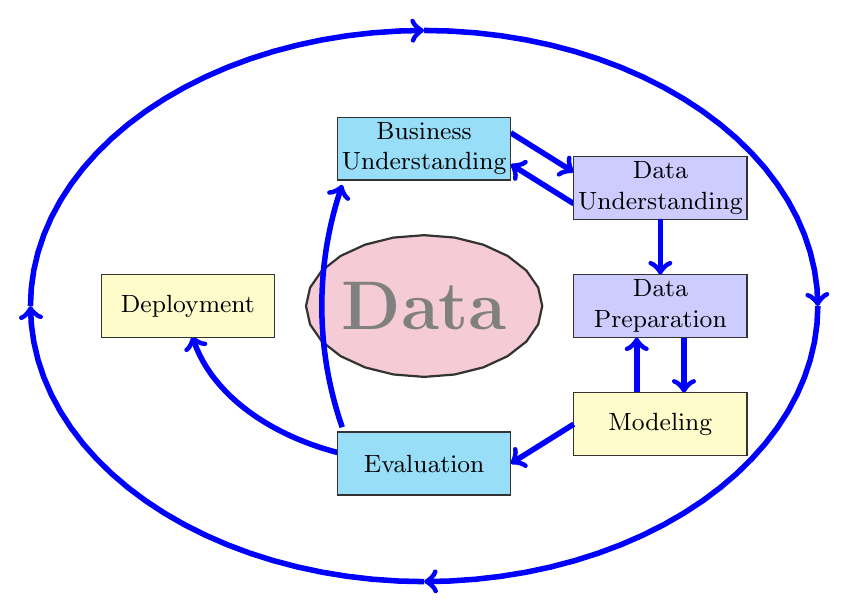
\begin{tikzpicture}
      
%      Cyan	#00FFFF	\definecolor{cyan}{rgb}{0.0, 1.0, 1.0}
    
    \draw [thick,domain=0:360,black!80, fill=blue!20!red!20] plot ({1.5*cos(\x)}, {0.9*sin(\x)});
    \node (D) at (0,0) {\Huge \textcolor{gray}{\textbf{Data}}};
    
    \draw [blue,line width = 2,domain=191:249,<-] plot ({3*cos(\x)}, {2*sin(\x)});

    \draw [blue,line width = 2,domain=160:200,<-] plot ({3+4.3*cos(\x)}, {4.5*sin(\x)});
    
    \draw [blue,line width = 2,->] (1.1, 2.2) -- (1.9,1.7);
    \draw [blue,line width = 2,<-] (1.1, 1.8) -- (1.9,1.3);
    \draw[black!80, fill=cyan!40] (-1.1,1.6) -- (1.1,1.6) -- (1.1,2.4) -- (-1.1,2.4) -- cycle;
    \node (BU) at (0,2) {\small \begin{tabular}{c} Business\\ Understanding \end{tabular}};
    
    
    \draw[black!80, fill=blue!20] (1.9,1.9) -- (4.1,1.9) -- (4.1,1.1) -- (1.9,1.1) -- cycle;
    \node (DP) at (3,1.5) {\small \begin{tabular}{c} Data\\ Understanding \end{tabular}};

    \draw [blue,line width = 2,->] (3, 1.1) -- (3,0.4);

    
    \draw[black!80, fill=blue!20] (1.9,0.4) -- (4.1,0.4) -- (4.1,-0.4) -- (1.9,-0.4) -- cycle;
    \node (DP) at (3,0) {\small \begin{tabular}{c} Data\\ Preparation \end{tabular}};

    \draw [blue,line width = 2,->] (3.3, -0.4) -- (3.3,-1.1);
    \draw [blue,line width = 2,<-] (2.7, -0.4) -- (2.7,-1.1);

    \draw[black!80, fill=yellow!20] (1.9,-1.9) -- (4.1,-1.9) -- (4.1,-1.1) -- (1.9,-1.1) -- cycle;
    \node (DP) at (3,-1.5) {\small Modeling};

    \draw [blue,line width = 2,<-] (1.1, -2) -- (1.9,-1.5);
    
    \draw[black!80, fill=cyan!40] (-1.1,-1.6) -- (1.1,-1.6) -- (1.1,-2.4) -- (-1.1,-2.4) -- cycle;
    \node (E) at (0,-2) {\small Evaluation};

    \draw[black!80, fill=yellow!20] (-1.9,0.4) -- (-4.1,0.4) -- (-4.1,-0.4) -- (-1.9,-0.4) -- cycle;
    \node (DP) at (-3,0) {\small \begin{tabular}{c} Deployment \end{tabular}};
    
    \draw [blue,line width = 2,domain=0:90,<-] plot ({5*cos(\x)}, {3.5*sin(\x)});
    \draw [blue,line width = 2,domain=90:180,<-] plot ({5*cos(\x)}, {3.5*sin(\x)});
    \draw [blue,line width = 2,domain=180:270,<-] plot ({5*cos(\x)}, {3.5*sin(\x)});
    \draw [blue,line width = 2,domain=270:360,<-] plot ({5*cos(\x)}, {3.5*sin(\x)});
  \end{tikzpicture}        
		\caption{Lebenszyklus eines Data Mining Projekts im CRISP-DM nach \cite{Chapman:2000}} 
		\label{CRISP-DM}
	\end{center}
\end{figure}

Auch dieses Modell betont, dass das eine Rückkehr zu zurückliegenden Phasen während des Prozesses wichtig ist. In Abbildung~\ref{CRISP-DM} sind nur die wichtigsten und häufigsten Verbindungen zwischen den Phasen dargestellt. Der äußere Kreis repräsentiert die zyklische Natur des Data-Mining-Prozesses selbst. \cite{Chapman:2000}

\section{Anwendungsnahe Prozessmodelle}

Die gezeigten Modelle bleiben sehr abstrakt und wenig auf tatsächliche technische Anwendungen im technischen Umfeld bezogen. Um die tatsächlichen Abläufe bei Verwendung verschiedener Systeme zur Wissensgenerierung und zur Verwendung im Feld abzubilden, können folgende Darstellungen hilfreich sein.

Für die Beschreibung von Projekten der künstlichen Intelligenz mit dem Jetson Nano wird ein modifiziertes KDD-Prozessmodell angenommen, das größtenteils dem Modell nach Fayyad entspricht, aber dennoch einige kleinere Veränderungen enthält. In Abbildung~\ref{KDDMod} ist dieses modifizierte Prozessmodell zu sehen.

\begin{figure}[H]
	\begin{center}
        
  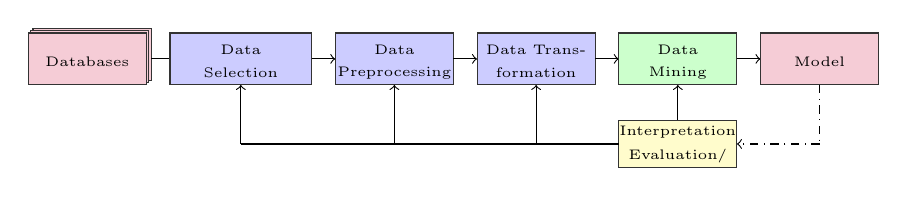
\begin{tikzpicture}[scale=0.6]
    \draw[draw, black!80, fill=blue!20!red!20]  (-2.90,0.10) rectangle (-0.40,1.20);
    \draw[draw, black!80, fill=blue!20!red!20]  (-2.95,0.05) rectangle (-.45,1.15);
    \draw[draw, black!80, fill=blue!20!red!20]  (-3,0) rectangle (-0.5,1.1);
    \node (AMP) at (-1.75,0.5) {\tiny Databases};
    
    %\visible<2->
    {
        \draw[->] (-0.4,0.55)--(1.5,0.55);
        \draw[draw, black!80, fill=blue!20]  (0,0) rectangle (3,1.1);
        \node (AMP) at (1.5,0.75) {\tiny Data};
        \node (AMP) at (1.5,0.25) {\tiny Selection};
    }
    
    %\visible<3->
    {
        \draw[->] (3,0.55)--(3.5,0.55);
        \draw[draw, black!80, fill=blue!20]  (3.5,0) rectangle (6,1.1);
        \node (AMP) at (4.75,0.75) {\tiny Data};
        \node (AMP) at (4.75,0.25) {\tiny Preprocessing};
    }
    
    
    %\visible<4->
    {
        \draw[->] (6,0.55)--(6.5,0.55);
        \draw[draw, black!80, fill=blue!20]  (6.5,0) rectangle (9,1.1);
        \node (AMP) at (7.75,0.75) {\tiny Data Trans-};
        \node (AMP) at (7.75,0.25) {\tiny formation};
    }
    
    %\visible<5->
    {
        \draw[->] (10.75,-1.25)--(10.75,0);
        \draw[->] (9.0,0.55)--(9.5,0.55);
        \draw[draw, black!80, fill=green!20]  (9.5,0) rectangle (12,1.1);
        \node (AMP) at (10.75,0.75) {\tiny Data};
        \node (AMP) at (10.75,0.25) {\tiny Mining};
    }
    
    {
%        \draw[->] (12,0.55)--(12.5,0.55);
        \draw[draw, black!80, fill=yellow!20]  (9.5,-1.75) rectangle (12,-0.75);
        \node (AMP) at (10.75,-1.0) {\tiny Interpretation};
        \node (AMP) at (10.75,-1.5) {\tiny Evaluation/};
    }
    
    \draw[->] (12,0.55)--(12.5,0.55);
    \draw[draw, black!80, fill=blue!20!red!20]  (12.5,0) rectangle (15,1.1);
    \node (AMP) at (13.75,0.5) {\tiny Model};
    
    
    %\visible<8->
    {
        \draw[-] (9.5,-1.25) -- (1.5,-1.25);
        \draw[->] (1.5,-1.25)--(1.5,0);
    }
    
    %\visible<9->
    {
        \draw[->] (4.75,-1.25)--(4.75,0);
        \draw[->] (7.75,-1.25)--(7.75,0);
    }
    
    %\visible<2->
    {
        \draw[dash dot,-] (13.75,0)--(13.75,-1.25);
        \draw[dash dot,->] (13.75,-1.25) -- (12,-1.25);
        
    }
  \end{tikzpicture}        
		\caption{Modifiziertes Modell des KDD-Prozess auf Grundlage des Modells nach \cite{Fayyad:1996}} 
		\label{KDDMod}
	\end{center}
\end{figure}

Die Linien zur Kennzeichnung der iterativen Schleifen sind durchgezogen und nicht gestrichelt, um die unbedingte Notwendigkeit dieser iterativen Korrekturschritte zu unterstreichen. Das Feedback vom Modell ist jedoch gestrichelt dargestellt, da in diesem Prozessmodell davon ausgegangen wird, dass das gewonnenen Wissen in Form eines Modells auf einem Edge-Computer, hier dem Jetson Nano, verwendet wird. Dies erschwert die direkt Rückmeldung und Korrekturen.

In Abbildung~\ref{KDDAnwendung} wird die Verteilung der Schritte auf verschiedene Ebenen sowie Lokalitäten und Systeme deutlich. Diese Darstellung bezieht sich auf die Anwendung im Umfeld einer Produktion. Denkbar wäre etwa die Erstellung eines Systems zur Prozesskontrolle, welches mit Hilfe einer Kamera fehlerhafte Werkstücke erkennt. Die Datenbasis würde mit eben dieser Kamera gesammelt werden. Die Verwendung der Daten inklusive der in den vorherigen
Abschnitten erläuterten Schritte erfolgt in einem Büro außerhalb der Produktion. Die gefundenen Ergebnisse kommen in dem Kontrollsystem aber wieder in der
Produktion zum Einsatz, wo sie neuen Daten ausgesetzt werden. Diese neuen Daten können in die Datenbank(en) aufgenommen werden und möglicherweise kann
auch eine Rückkopplung zwischen den Ergebnissen im Feld zu einer im Büro stattfindenden Überprüfung und Korrektur der Modelle realisiert werden.

\begin{figure} [H]
\begin{center}   
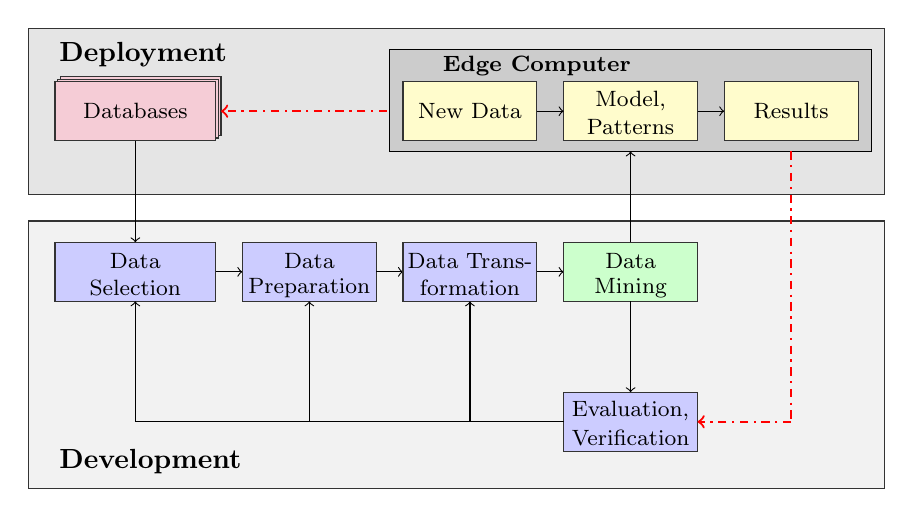
\begin{tikzpicture}[scale=0.68]
    \draw[draw, black!80, fill=black!10]  (-0.5,2) rectangle (15.5,5.1);
    
    \node[right] at (-0.1,4.6) {\textbf{Deployment}};
    
    \draw[draw, black!80, fill=black!5]  (-0.5,-3.5) rectangle (15.5,1.5);
    
    \node[right] at (-0.1,-3) {\textbf{Development}};
    
    
    \draw[draw, black!80, fill=blue!20!red!20]  (0.10,3.10) rectangle (3.10,4.20);
    \draw[draw, black!80, fill=blue!20!red!20]  (0.05,3.05) rectangle (3.05,4.15);
    \draw[draw, black!80, fill=blue!20!red!20]  (0,3) rectangle (3,4.1);
    \node (AMP) at (1.5,3.55) {\footnotesize Databases};
    
    %\visible<2->
    {
        \draw[->] (1.5,3)--(1.5,1.1);
        \draw[draw, black!80, fill=blue!20]  (0,0) rectangle (3,1.1);
        \node (AMP) at (1.5,0.75) {\footnotesize Data};
        \node (AMP) at (1.5,0.25) {\footnotesize Selection};
    }
    
    %\visible<3->
    {
        \draw[->] (3,0.55)--(3.5,0.55);
        \draw[draw, black!80, fill=blue!20]  (3.5,0) rectangle (6,1.1);
        \node (AMP) at (4.75,0.75) {\footnotesize Data};
        \node (AMP) at (4.75,0.25) {\footnotesize Preparation};
    }
    
    
    %\visible<4->
    {
        \draw[->] (6,0.55)--(6.5,0.55);
        \draw[draw, black!80, fill=blue!20]  (6.5,0) rectangle (9,1.1);
        \node (AMP) at (7.75,0.75) {\footnotesize Data Trans-};
        \node (AMP) at (7.75,0.25) {\footnotesize formation};
    }
    
    %\visible<5->
    {
        \draw[->] (9.0,0.55)--(9.5,0.55);
        \draw[draw, black!80, fill=green!20]  (9.5,0) rectangle (12,1.1);
        \node (AMP) at (10.75,0.75) {\footnotesize Data};
        \node (AMP) at (10.75,0.25) {\footnotesize Mining};
    }
    
    %\visible<6->
    {
        \draw[fill=black!20] (6.25,2.8)--(6.25,4.7) -- (15.25,4.7) -- (15.25,2.8) -- cycle;

        \node (AMP) at (9,4.4) {\footnotesize \textbf{Edge Computer}};
        
        \draw[->] (10.75,1.1)--(10.75,2.8);
        \draw[draw, black!80, fill=yellow!20]  (9.5,3) rectangle (12,4.1);
        \node (AMP) at (10.75,3.75) {\footnotesize Model,};
        \node (AMP) at (10.75,3.25) {\footnotesize Patterns};
    }
    
    {
        \draw[->] (9,3.55)--(9.5,3.55);
        \draw[draw, black!80, fill=yellow!20]  (6.5,3) rectangle (9,4.1);
        \node (AMP) at (7.75,3.55) {\footnotesize New Data};
    }
    
    {
        \draw[->] (12,3.55)--(12.5,3.55);
        \draw[draw, black!80, fill=yellow!20]  (12.5,3) rectangle (15,4.1);
        \node (AMP) at (13.75,3.55) {\footnotesize Results};
    }
    
    %\visible<7->
    {
        \draw[->] (10.75,0)--(10.75,-1.7);
        \draw[draw, black!80, fill=blue!20]  (9.5,-2.8) rectangle (12,-1.7);
        \node (AMP) at (10.75,-2.05) {\footnotesize Evaluation,};
        \node (AMP) at (10.75,-2.55) {\footnotesize Verification};
    }
    
    %\visible<8->
    {
        \draw[-] (9.5,-2.25) -- (1.5,-2.25);
        \draw[->] (1.5,-2.25)--(1.5,0);
    }
    
    %\visible<9->
    {
        \draw[->] (4.75,-2.25)--(4.75,0);
        \draw[->] (7.75,-2.25)--(7.75,0);
    }
    
    %\visible<2->
    {
        \draw[red, thick, dash dot,-] (13.75,2.8)--(13.75,-2.2);
        \draw[red,thick, dash dot,->] (13.75,-2.25) -- (12,-2.25);
        
        \draw[red,thick, dash dot,->] (6.2,3.55) -- (3.1,3.55);
    }
  \end{tikzpicture}
  \caption{KDD-Prozess im industriellen Umfeld}\label{KDDAnwendung}
\end{center}
\end{figure}


\section{Rolle des Anwenders}

Brachman und Anand \cite{Brachman:1994} kritisieren, dass die üblichen Definitionen des KDD zu sehr auf die resultierenden Informationen fokussiert sind und dabei die Komplexität des Prozesses nicht angemessenen widerspiegeln. Demnach müsse die Rolle des Menschen stärker betont werden, auch wenn es langfristig das Bestreben hin zu vollständig autonomen Integrierungen des KDD-Prozesses gebe. Die Front-End-Anforderungen müssen erkannt und miteinander in Einklang gebracht werden und auch die Datenaufbereitung, Analyse und Auswertung sowie Überwachung der einzelnen Schritte durch Visualisierung setzen Domänenwissen des Anwenders und sein Eingreifen voraus. Zur Unterstützung empfehlen die Autoren eine entsprechende Arbeitsumgebung (Knowldege Discovery Support Environment), die einen einfachen Datenaustausch zwischen den verschiedenen Arbeitsschritten erlaubt sowie die Wiederverwendung schon geschaffener Strukturen erleichtert. Außerdem könnte ein System den Anwender bei der Auswahl passender Methodik unterstützen.

\section{KDD-Prozess am Beispiel der Bild-Klassifizierung mit dem Jetson Nano} \label{BeispielKDD}

Um den Prozess in Bezug auf eine greifbare Anwendung zu betrachten, soll als Beispiel die Entwicklung einer Bild-Klassifizierung mit dem Jetson Nano als KDD-Prozess beleuchtet werden.

\subsection{Daten}


Als Datengrundlage für eine Bildklassifizierung müssen ausreichend viele Bilder inklusive ihrer im Sinne der Anwendung korrekten Klassifizierung, dem Label, zur Verfügung stehen. Es gibt verschiedene Bild-Datenbank, die frei zugänglich sind, darunter zum Beispiel ImageNet, MS-COCO und CIFAR-10. Natürlich kommen nur solche Datenbanken infrage, die Objekte und Merkmale enthalten, die das Modell später erkennen soll. \cite{Deng:2009,Deng:2012,Schutten:2016,Agarap:2018b} 

Auch Dateiformate und Farbtiefe sowie Anzahl an Farbkanälen sollten bei der Suche nach geeigneten Datenbanken bereits berücksichtigt werden, da nicht in jedem Fall eine (verlustfreie) Transformation zu den benötigten Dateiformaten möglich ist oder in der Datenbank weniger Informationen als gewünscht enthalten sein könnten. Welche Dateiformate, Farbtiefen und Farbkanäle zu verwenden sind, hängt von der gewünschten Anwendung, der verwendeten Trainingsplattform und des verwendeten Algorithmus' ab.

\subsection{Datenauswahl}

Aus den identifizierten, zur Verfügung stehenden und für die Anwendung verwendbaren Datenbanken können nun die zu verwendenden Bilder ausgewählt werden. Beispielsweise könnte eine Datenbank in ihrer Gesamtheit verwendet werden, es kann aber auch nur ein Teil einer solchen verwendet oder mehrere Datenbanken kombiniert werden. Immens wichtig ist dabei, dass alle Klassen, die erkannt werden sollen, auch in den ausgewählten Daten vorhanden sind. Wie viele Bilder ausgewählt werden, hängt von dem geplanten Umfang des Trainings und der Test ab, was maßgeblichen Einfluss auf die Trainingszeit, aber unter Umständen auch auf die Performance des erzielten Modells hat. 


\subsection{Vorverarbeitung}

Bei der Datenvorbereitung geht es meist primär um die Datenreinigung. Dies beinhaltet vor allem das Entfernen von Ausreißern. In Bezug auf Bilder sind diese Ausreißer vor allem verrauschte oder schlecht aufgelöste Bilder. Diese sollten entfernt oder mit passenden Algorithmen aufbereitet werden. Bei Verwendung von Bildern aus den bekannten Open-Source-Bilddatenbanken, wie ImageNet \cite{Deng:2009},  sollte die Bildqualität kein Problem sein.

Des Weiteren müssen die Bilder in das Format konvertiert werden, das von der jeweiligen Plattform unterstützt wird. Dabei ist zu berücksichtigen, dass komprimierte Dateiformate nicht immer verlustfrei dekomprimiert werden können.

\subsection{Transformation}

Schließlich müssen die Bilder in eine Darstellung transformiert werden, die im Data Mining verwendet werden kann. Eventuell muss die Farbtiefe je Kanal oder die Anzahl der Kanäle angepasst werden. Unter Umständen muss ein RGB-Bild in ein Graustufenbild überführt werden. Gängig ist zudem eine Normalisierung der Bilder, etwa auf den Mittelwert 0 und Standardabweichung 1.

Der Algorithmus, der für die Phase Data Mining gewählt wurde, bestimmt auch das Eingabeformat der Daten. Auf Bilder angewandt bedeutet dies, welches Dateiformat zu verwenden ist. Neben dem Dateiformat ist aber die Farbauflösung die Anzahl der Pixel festgelegt. In dieser Phase werden die Bilder entsprechend angepasst.


\subsection{Data Mining}

Im Schritt des Data Minings findet die eigentliche Modellbildung statt. Dazu muss zuerst der Algorithmus gewählt werden beziehungsweise die Architektur definiert und das Modell dementsprechend aufgebaut werden. Wenn Deep Learning-Algorithmen verwendet werden, so muss die Architektur definiert. Mit der Definition der Architektur werden die Hyperparamter festgelegt.  Dann kann der Algorithmus mit den ausgewählten Bildern trainiert werden. Beim Training werden die Gewichte optimiert. Ihre Anpassung erfolgt dabei auf Grundlage der Trainingsbilder. Nach einer vorgegebenen Anzahl an Trainingsbildern werden die Validierungsbilder zum Test der Genauigkeit des aktuellen Modells genutzt. Nach mehreren Epochen, also mehreren Durchläufen aller Trainingsbilder, kann das Modell getestet werden.

\subsection{Evaluation/Verifikation}

Die Interpretation und Bewertung des trainierten Modells erfolgt in erster Instanz immer wieder während des Trainings mit Hilfe des Validierungsdatensatzes. In zweiter Instanz wird das Modell direkt nach dem Training mit Hilfe der dem Modell noch unbekannten Testbilder getestet. Sind die erzielten Ergebnisse zufriedenstellend, kann das Modell in die Anwendung integriert werden. Auch in dieser Instanz ist es wichtig, die Performance des Modells zu testen, um eventuell Rückschlüsse ziehen und Korrekturen vornehmen zu können. In der dynamischen Anwendung herrschen andere Rahmenbedingungen, sodass die Rückschlüsse auf notwendige Korrekturen in den vorangegangenen Schritten großes Domänenwissen erfordern kann.

Die Interpretation des gefundenen Modells ist für neuronale Netze, insbesondere für komplexe Netze wie \ac{cnn}, nicht trivial. Es können unter Umständen keine direkten Zusammenhänge extrahiert werden, die sich auf andere Anwendungen übertragen ließen.

\subsection{Model}

Das trainierte Modell kann schließlich in der vorgesehenen Anwendung integriert werden. Während die Datenvorbereitung und das Training auf einem Rechner stattfinden, der im Allgemeinen mit einer hochen Rechenleistung ausgestattet ist, soll das Modell auf einem Edge-Computer wie dem Jetson Nano verwendet werden. So könnte beispielsweise eine Echtzeit-Objekterkennung mit einer an den Jetson Nano angeschlossenen Kamera auf Grundlage des Trainings mit den statischen Bildern erfolgen. Unter Umständen ist zum Transfer des Modells auf den Edge-Computer eine Überführung des Modells in ein anderer Format notwendig.


\section{Datenanalyse- und Data-Mining-Verfahren im Überblick}

Im folgenden soll ein Überblick über einige Verfahren des Data Minings gegeben werden.

\subsection{Definition Datenanalyse}


Die Datenanalyse versucht mit Hilfe statistischer Methoden Informationen aus großen Datenmengen zu gewinnen und diese im Anschluss zu visualisieren. Das komplexe Gebiet der Datenanalyse lässt sich in die Bereiche der deskriptiven, der inferenziellen, der explorativen und konfirmatorischen Datenanalyse unterteilen. Bei der deskriptiven Datenanalyse werden die Informationen der Einzeldaten, welche beispielsweise einer Totalerhebung entnommen wurden, so verdichtet und dargestellt, dass das Wesentliche deutlich wird. Liegen lediglich die Daten einer Stichprobenerhebung (Teilerhebung) zu Grunde, so ruht der Schwerpunkt der Datenanalyse auf der Übertragung der Stichprobenbefunde auf die Grundgesamtheit. Dabei wird von einer inferenziellen Datenanalyse gesprochen. Bei der explorativen Datenanalyse geht es darum, die verfügbare Datenmenge so zu verarbeiten, dass Strukturen in den Daten sowie Zusammenhänge ebendieser aufgezeigt und in besonderem Maße hervorgehoben werden können. Im Gegensatz dazu ist das Ziel der konfirmatorischen Datenanalyse die Überprüfung von Zusammenhängen.

\subsection{Statistischen Datenanalyse}

Bei der statistischen Datenanalyse wird in der Regel mit den Berechnungen des Mittelwertes und der Standardabweichung (oder Varianz) begonnen. Außerdem erfolgt die Prüfung der Daten auf Normalverteilung.

\subsubsection{Hypothesentest}

Für die Anwendung des Hypothesentests werden immer zwei Hypothesen formuliert: eine Nullhypothese $H_0$, die meistens beinhaltet, dass die vermutete Datenstruktur nicht existiert und die Alternativhypothese $H_1$ bzw. $H_A$, die meistens beinhaltet, dass die vermutete Datenstruktur existiert. Der Hypothesentest bezieht sich auf die Annahme einer wahren Nullhypothese \cite{Akremi:2011}. Es muss bewiesen werden, dass die Nullhypothese falsch ist. Zuerst werden Werte wie der T-Wert („Der T-Wert ergibt sich aus dem Quotienten des arithmetischen Mittels der Differenzen zwischen zwei zu vergleichenden Variablen und dem Schätzwert des Standardfehlers für dieses Mittel in der Grundgesamtheit.“ \cite{Akremi:2011}) oder der F-Wert berechnet. Diese Werte werden mit einem der Situation angepassten kritischen Wert verglichen. Ist dieser berechnete Wert kleiner als der kritische Wert, gilt die Nullhypothese als wahr. In diesem Fall ist auch der P-Wert, also die Wahrscheinlichkeit, mit der das auf die Nullhypothese bezogene Ergebnis eintritt, nur wenig kleiner als 0,05. Ist der P-Wert hingegen sehr klein, wird die Nullhypothese verworfen. Es gilt als relativ sicher, dass die Nullhypothese falsch ist; jedoch ist nicht bekannt, welche Hypothese richtig ist. Wird die Nullhypothese nicht verworfen, darf im Umkehrschluss nicht auf die Richtigkeit ebendieser geschlossen werden \cite{Akremi:2011}. In diesem Fall kann das Ergebnis nicht interpretiert werden.

\subsubsection{Normalverteilung, P-Test, T-Test}

Der P-Wert (Signifikanzwert) gibt an, wie extrem der auf der Basis der erhobenen Daten berechnete Wert der Teststatistik ist. Außerdem deutet er an, wie wahrscheinlich es ist, ein solches Stichprobenergebnis oder ein noch extremeres zu erhalten, wenn die Nullhypothese wahr ist. Da der Wert ein Wahrscheinlichkeitswert ist, nimmt er Werte zwischen Null und Eins an. Mit dem P-Wert wird deshalb angedeutet, wie extrem das Ergebnis ist: je kleiner der P-Wert, desto mehr spricht das Ergebnis gegen die Nullhypothese. Üblicherweise wird vor dem Test ein Signifikanzniveau $\alpha$ festgelegt und die Nullhypothese dann verworfen, wenn der P-Wert kleiner oder gleich $\alpha$ ist \cite{Akremi:2011}. Um Entscheidungen treffen zu können, ob die Nullhypothese abgelehnt oder beibehalten werden soll, haben sich feste Grenzen etwa bei 5 \%, 1 \% oder 0,1\% etabliert. Wenn die Nullhypothese verworfen wird, wird das Resultat als statistisch signifikant bezeichnet. Die Größe des P-Werts gibt keine Aussage über die Größe des wahren Effekts.

Der T-Test bezeichnet eine Gruppe von Hypothesentests mit T-verteilter Testprüfgröße \cite{Akremi:2011}, die aber häufig nach Einstichproben-T-Test und Zweistichproben-T-Test unterschieden wird. Voraussetzung für die Durchführung des T-Tests ist die Normalverteilung der zu untersuchenden Grundgesamtheit der Daten. Des Weiteren muss ein genügend großer Stichprobenumfang vorliegen. Sind die Daten nicht normalverteilt, kann der T-Test nicht angewendet werden und es wird nach dem Prinzip des U-Tests verfahren. Beim Einstichproben-T-Test wird mit Hilfe des Mittelwertes einer Stichprobe geprüft, ob sich der Mittelwert der Grundgesamtheit von einem vorgegebenen Sollwert unterscheidet. Der klassische T-Test (Zweistichproben-T-Test) hingegen prüft, ob sich Mittelwerte zweier unabhängiger Stichproben wie die Mittelwerte zweier Grundgesamtheiten zueinander verhalten. Dabei wird vorausgesetzt, dass beide Stichproben aus Grundgesamtheiten gleicher Varianz entstammen. Die Varianz ist das Quadrat der Standardabweichung. Je größer die Varianz ist, desto flacher verläuft die Normalverteilungskurve. Werden zwei Stichprobengrößen miteinander verglichen, muss zusätzlich die gewichtete Varianz ermittelt werden. Dabei hat die größere Stichprobe den entscheidenderen Einfluss auf das Ergebnis.

\subsubsection{ANOVA (Analysis of Variance)}

\glqq Die Varianzanalyse, im Deutschen zumeist ANOVA genannt, sucht primär nach Unterschieden zwischen Gruppen und testet, ob das Aufteilen der Daten in unterschiedliche Gruppen die unerklärte Variabilität reduziert.\grqq \cite{Dormann:2013} Voraussetzungen für die Varianzanalyse sind die normalverteilten Werte in jeder Gruppe, die annähernde Gleichheit der Standardabweichungen sowie die Unabhängigkeit der Messwerte voneinander. Es wird geprüft, ob sich die Mittelwerte mehrerer Gruppen unterscheiden. Im einfachsten Fall lautet die Nullhypothese: Die Mittelwerte aller Gruppen sind gleich. Dann ergibt sich folgende Alternativhypothese: Nicht alle Mittelwerte sind gleich. Mit den Prüfgrößen des Verfahrens wird getestet, ob die Varianz zwischen den Gruppen größer ist als die Varianz innerhalb der Gruppen. Dadurch kann ermittelt werden, ob die Gruppeneinteilung sinnvoll ist oder nicht bzw. ob sich die Gruppen signifikant unterscheiden oder nicht. Die Varianzanalyse ist in ihrer einfachsten Form eine Alternative zum T-Test. Das Ergebnis ist das gleiche wie beim T-Test, \glqq denn die Ergebnisse einer einfaktoriellen Varianzanalyse (one-way ANOVA) und eines T-Tests sind identisch, wenn die beiden Stichproben die gleiche Varianz haben.\grqq \cite{Dormann:2013}

\subsection{Methoden und Verfahren des Data-Minings im Überblick}


Typische Methoden des Data-Mining sind:

\begin{itemize}
  \item Clusteranalyse: Gruppierung von Objekten aufgrund von Ähnlichkeiten,
  \item Klassifikation: Elemente werden den bestehenden Klassen zugeordnet,
  \item Assoziationsanalyse: Identifizierung von Zusammenhängen und Abhängigkeiten in den Daten,
  \item Regressionsanalyse: Identifizierung von Beziehungen zwischen Variablen,
  \item Ausreißererkennung: Identifizierung von ungewöhnlichen Datensätzen,
  \item Korrelationsanalyse: Untersucht die Beziehung zwischen zwei Variablen,
  \item Zusammenfassung: Transformation des Datensatzes in eine kompaktere Beschreibung ohne wesentlichen Informationsverlust.
\end{itemize}

\bigskip

Dabei zählen die Ausreißererkennung sowie die Clusteranalyse zu den Beobachtungsproblemen; Klassifikation und Regressionsanalyse zählen zu den Prognoseproblemen.

\subsubsection{Clusteranalyse \& Klassifikation}

Mit Hilfe der Clusteranalyse sollen Ähnlichkeitsstrukturen in großen Datenbeständen aufgezeigt werden, mit dem Ziel, neue Gruppen in den Daten zu identifizieren. Die gefundenen Ähnlichkeitsgruppen können graphentheoretisch, hierarchisch, partitionierend oder optimierend sein. Die einem Cluster zugeordneten Objekte sollen dabei möglichst homogen sein, die unterschiedlichen Clustern zugeordneten Objekte sollen sehr stark heterogen sein \cite{Janssen.2007}. Außerdem können bei der Clusterbildung mehrere Merkmale parallel herangezogen werden. Die Clusteranalyse erfolgt in den nachfolgenden Schritten.
	
Zu Beginn wird jedes Objekt als einzelner Cluster betrachtet. Danach werden die beiden Einzelobjekte, die sich am ähnlichsten sind, miteinander vereinigt. Die Vereinigung reduziert die Clusteranzahl um Eins. Danach werden wiederum alle Distanzen der einzelnen Objekte berechnet und die beiden Objekte mit dem kleinsten Abstand zu einem neuen Cluster zusammengefasst. Dies könnte theoretisch solange wiederholt werden, bis alle Objekte in einem einzigen Cluster, einem sogenannten Megacluster, vereinigt sind. Für die Analyse der Daten ist es jedoch viel bedeutsamer, die am sinnvollsten erscheinende Clusterung zu ermitteln. Die Clusteranzahl wird durch die Betrachtung der Varianz innerhalb und zwischen den Gruppen bestimmt. Es wird festgelegt, welche Clusterung am sinnvollsten erscheint, da für die Funktion selbst keine Abbruchbedingung vorgegeben ist. In der Regel sind verschiedene Clustereinteilungen von Vorteil.
	
Voraussetzungen für die Anwendung der Clusteranalyse sind die metrisch skalierten Merkmale, welche einfach in die Analyse einfließen können; ordinal und nominal skalierte Merkmale müssen als Dummy-Variablen \cite{Janssen.2007} skaliert werden. Merkmale, die in unterschiedlichen Dimensionen skaliert sind, können zu einer Ergebnisverzerrung führen. Diese Werte müssen vor der Durchführung einer Clusteranalyse, zum Beispiel durch eine Z-Transformation \cite{Janssen.2007}, standardisiert werden. Des Weiteren sollten die Merkmale nicht untereinander korrelieren.
	
Die Distanz zwischen zwei Einzelobjekten wird durch das Distanzmaß bestimmt. Je größer das Maß, desto unähnlicher sind sich die Objekte. Die verschiedenen Clustermethoden \cite{Janssen.2007} dienen der Bestimmung der Distanz zwischen zwei Clustern oder einem Cluster und einem Einzelobjekt. Bei der Klassifikation hingegen werden die Daten bereits bestehenden Gruppen zugeordnet.
	
\subsubsection{Assoziationsanalyse \& Regressionsanalyse}

\glqq Durch eine Assoziationsanalyse werden Regeln generiert, welche die Beziehungen zwischen den in den Datensätzen eines Datenbestandes vorkommenden Elementen (Items) beschreiben.\grqq \cite{Gluchowski:2006} Diese Abhängigkeiten werden in der Form Wenn Item $A$, dann Item $B$ bzw. $A \rightarrow B$  dargestellt. Ein Item ist dabei die Ausprägung eines Attributwertes eines Datensatzes. Ein Beispiel für eine einfache Regel wäre: Wenn ein Kunde Bier kauft, dann kauft er in 70 Prozent der Fälle auch Chips. Diese Beziehungen werden nicht als Hypothesen angenommen, sondern sollen mit der Assoziationsanalyse aus den Daten entdeckt werden. Erst nachdem ein auffälliges Muster gefunden wurde, wird untersucht, ob es sich wirklich um eine Abhängigkeit handelt und falls ja, werden Assoziationsregeln dazu aufgestellt. Kenngrößen von Assoziationsregeln sind Support, Konfidenz und Lift. \glqq Je größer der Supportwert ist, desto relevanter ist die Regel.\grqq \cite{Gluchowski:2006}
	
Die Regressionsanalyse ist das Analyseverfahren zur Errechnung einer Regression in Form einer Regressionsgeraden bzw. -funktion. Die Regression gibt an, welcher gerichtete lineare Zusammenhang zwischen zwei oder mehreren Variablen besteht \cite{Gluchowski:2006}. Das Bestimmtheitsmaß (R²) drückt dabei aus, wie gut die Regressionsgerade den Zusammenhang zwischen unabhängiger und abhängiger Variable wiedergibt. R² liegt zwischen 0 und 1, wobei der Wert R² = 1 bedeuten würde, dass jeder beobachtete Datenpunkt direkt auf der Regressionsgeraden liegt. Durch die Ermittlung einer Regressionsfunktion kann noch keine Aussage über die Signifikanz eines Zusammenhangs getroffen werden. Die Signifikanz der Regression wird durch den F-Test ermittelt.

Zu Beginn der Regressionsanalyse steht die Aufbereitung der Daten. Fehlende Daten werden weggelassen bzw. aufgefüllt, Daten werden transformiert und die Interaktionen (bei linearer Regression) werden berücksichtigt. Mittels mathematischer Verfahren wird eine Funktion f ermittelt, so dass die Residuen e minimal werden (Residuen: Differenz zwischen einer Regressionsgeraden und den Messwerten \cite{Kaehler:2011}). Die Modellvalidierung, also die Überprüfung ob das Modell eine gute Beschreibung des Zusammenhangs ist, umfasst die
	
\begin{itemize}
  \item Residuenanalyse,
  \item Überanpassung,
  \item Untersuchung der Daten auf Ausreißer und einflussreiche Datenpunkte und
  \item Multikollinearität der unabhängigen Variablen.
\end{itemize}	

\bigskip
Das validierte Modell kann zur Prognose von Werten von y bei gegebenen Werten von x herangezogen werden. Zur Abschätzung der Unsicherheit der Prognose wird neben dem prognostizierten y-Wert häufig auch ein Konfidenzintervall angegeben.


\subsubsection{Ausreißererkennung}

Ausreißer sind Messwerte oder Befunde, die inkonsistent zu dem Rest der Daten sind, beispielsweise indem sie ungewöhnliche Attributwerte haben oder nicht den Erwartungen entsprechen. Die Erwartung ist meistens der Streuungsbereich um den Erwartungswert herum, in dem sich die meisten Messwerte befinden. \glqq Robuste Grenzen für die Erkennung von Ausreißern für viele Verteilungstypen können auch auf der Grundlage der Quartile und der Quartildistanz abgeleitet werden.\grqq \cite{Sachs.2006} Werte explorativer Studien, die weiter als das 1,5-fache des Quartilabstandes außerhalb dieses Intervalls liegen, werden als Ausreißer bezeichnet. Im Boxplot werden besonders hohe Ausreißer gesondert dargestellt.

Das Verfahren Local Outlier Factor sucht beispielsweise Objekte, die eine von ihren Nachbarn deutlich abweichende Dichte aufweisen, dann wird an dieser Stelle von dichtebasierter Ausreißererkennung gesprochen. Identifizierte Ausreißer werden anschließend meist manuell verifiziert und aus dem Datensatz ausgeblendet, da sie die Ergebnisse anderer Verfahren verschlechtern können. Vor einer Entscheidung zugunsten der Entfernung von Werten ist daher in jedem Fall noch zu überprüfen, welcher Datenverlust bei der Löschung oder Kennzeichnung der fehlenden Werte entsteht. Sinkt die Zahl der verfügbaren Datensätze unter das zum Fortfahren notwendige Niveau, so ist das Entfernen der Ausreißer zu vermeiden.
	
\subsubsection{Korrelationsanalyse}

Eine wichtige Aufgabe der Datenanalyse ist die Analyse des Zusammenhangs zwischen einzelnen Merkmalen. Die Stärke des Zusammenhangs von zwei quantitativen Merkmalen wird in der deskriptiven Statistik und Inferenzstatistik als Korrelation bezeichnet und kann in lineare und nichtlineare Korrelation unterschieden werden. Bei multivariaten Datensätzen wird zusätzlich für jedes Paar von Variablen der Korrelationskoeffizient berechnet.\cite{Goettingen} \glqq Zur Korrelationsanalyse werden vornehmlich Verfahren der klassischen, multivariaten, robusten und explorativen Statistik eingesetzt, aber auch verschiedenste nichtlineare Regressionsverfahren, deren Approximationsfehler als Korrelationsmaß verwendet werden können.\grqq \cite{Runkler.2015} Voraussetzung für die Durchführung der Korrelationsanalyse ist die Normalverteilung der untersuchten Daten.
	
\subsubsection{Zusammenfassung als Methode des Data-Minings}

Durch die Transformation eines Datensatzes in eine kompaktere Beschreibung seiner Informationen, gewährleistet die Zusammenfassung eine verlustfreie Darstellung wesentlicher Information. Die Zusammenfassung erfolgt textuell, visuell oder kombiniert.



%
%[1] Vgl. Akremi, L., Baur, N., Fromm, S. (Hrsg.), Datenanalyse mit SPSS für Fortgeschrittene 1 – Datenaufbereitung und uni- und bivariate Statistik, 3., überarbeitete und erweiterte Auflage, Springer Fachmedien, Wiesbaden, 2011, S. 247.
%[2] „Der T-Wert ergibt sich aus dem Quotienten des arithmetischen Mittels der Differenzen zwischen zwei zu vergleichenden Variablen und dem Schätzwert des Standardfehlers für dieses Mittel in der Grundgesamtheit.“ Zitiert aus Akremi, L., Baur, N., Fromm, S. (Hrsg.), 2011, S. 267.
%[3] Vgl. Akremi, L., Baur, N., Fromm, S. (Hrsg.), Datenanalyse mit SPSS für Fortgeschrittene 1 – Datenaufbereitung und uni- und bivariate Statistik, 3., überarbeitete und erweiterte Auflage, Springer Fachmedien, Wiesbaden, 2011, S. 200.
%[4] Vgl. Akremi, L., Baur, N., Fromm, S. (Hrsg.), Datenanalyse mit SPSS für Fortgeschrittene 1 – Datenaufbereitung und uni- und bivariate Statistik, 3., überarbeitete und erweiterte Auflage, Springer Fachmedien, Wiesbaden, 2011, S. 203.
%[5] Vgl. Akremi, L., Baur, N., Fromm, S. (Hrsg.), Datenanalyse mit SPSS für Fortgeschrittene 1 – Datenaufbereitung und uni- und bivariate Statistik, 3., überarbeitete und erweiterte Auflage, Springer Fachmedien, Wiesbaden, 2011, S. 257.
%[6] Zitiert aus Dormann, C., Parametrische Statistik – Verteilungen, miximum likelihood und GLM in R, 2., überarbeitete und erweiterte Auflage, Springer-Verlag, Berlin, 2013, S. 199.
%[7] Zitiert aus Dormann, C., Parametrische Statistik – Verteilungen, miximum likelihood und GLM in R, 2., überarbeitete und erweiterte Auflage, Springer-Verlag, Berlin, 2013, S. 202.
%[8] Zitiert aus Hung, P. T., Data-Mining und KDD – ein Überblick, TU Dresden, 2009, S. 3.
%[9] Vgl. Hung, P. T., Data-Mining und KDD – ein Überblick, TU Dresden, 2009, S. 9.
%[10] Vgl. Queckbörner, S., Was ist Data Mining?, Technische Universität Kaiserslautern, o. J., S. 7.
%
%[11] Vgl. Böhm, Chr., Vorlesung „Knowledge Discovery in Databases“, Ludwig Maximilians Universität München, Institut für Informatik, Lehr- und Forschungseinheit für Datenbanksysteme, München, 2003, S. 7.
%[12] Vgl. Böhm, Chr., Vorlesung „Knowledge Discovery in Databases“, Ludwig Maximilians Universität München, Institut für Informatik, Lehr- und Forschungseinheit für Datenbanksysteme, München, 2003, S. 15.
%[13] Vgl. Janssen, J., Laatz, W., Statistische Datenanalyse mit SPSS für Windows, 6., neu bearbeitete und erweiterte Auflage, Springer-Verlag, Berlin, Heidelberg, 2007, S. 487.
%[14] Vgl. Janssen, J., Laatz, W., Statistische Datenanalyse mit SPSS für Windows, 6., neu bearbeitete und erweiterte Auflage, Springer-Verlag, Berlin, Heidelberg, 2007, S. 448.
%[15] Vgl. Janssen, J., Laatz, W., Statistische Datenanalyse mit SPSS für Windows, 6., neu bearbeitete und erweiterte Auflage, Springer-Verlag, Berlin, Heidelberg, 2007, S. 226.
%[16] Vgl. Janssen, J., Laatz, W., Statistische Datenanalyse mit SPSS für Windows, 6., neu bearbeitete und erweiterte Auflage, Springer-Verlag, Berlin, Heidelberg, 2007, S. 489.
%[17] Zitiert aus Gluchowski, P., F., Chamoni, P., Analytische Informationssysteme: Business Intelligence-Technologien und -Anwendungen 3., vollst. überarb. Auflage, 2006, S. 276.
%[18] Zitiert aus Gluchowski, P., Chamoni, P., Gluchowski, P., F., Chamoni, P., Analytische Informationssysteme: Business Intelligence-Technologien und -Anwendungen 3., vollst. überarb. Auflage, 2006, S. 277.
%[19] Vgl. Gluchowski, P., Chamoni, P., Gluchowski, P., F., Chamoni, P., Analytische Informationssysteme: Business Intelligence-Technologien und -Anwendungen 3., vollst. überarb. Auflage, 2006, S. 276.
%[20] Residuen: Differenz zwischen einer Regressionsgeraden und den Messwerten, vgl. Kähler, W.-M., 2011, S. 139.
%[21] Zitiert aus Sachs, L., Hedderich, J., Angewandte Statistik – Methodensammlung mit R, 12., vollständig neu bearbeitete Auflage, Springer-Verlag, Berlin, Heidelberg, 2006, S. 344.
%[22] Vgl. o.A., Uni Göttingen, Kapitel 3: Erste Schritte der Datenanalyse, Göttingen, o. J., S. 23.
%[23] Zitiert aus Runkler, T. A., Data Mining – Modelle und Algorithmen intelligenter Datenanalyse, 2., aktualisierte Auflage, Springer Fachmedien, Wiesbaden, 2015, S. 59.